%%% 3Background / %%%
\chapter{Background} \label{ch:background}
%To understand the interpretation of interaction graph and design of endorsement
%model, basic concepts about graph properties and metrics is required.
%Similarly, Blockchain relies a lot on cryptographic functions to maintain its
%property of the secure, immutable and attack-resilient structure. This chapter,
%therefore, provides a general overview of the background concepts that is
%required for the subsequent sections. 
Trust and reputation can be used across several domains, and their definitions
vary depending on context. It is essential to recognize the context in which
this term is being used. Similarly, blockchain can be seen as a relatively new
technology although the underlying sets of cryptographic functions it uses have
been around for a long time. Blockchain technology is being researched both by
academia and industry to explore its possibilities and in diverse use cases,
e.g., as a privacy-preserving smart contract~\cite{kosba2016hawk} or as a way
to protect personal data~\cite{zyskind2015decentralizing}. This chapter aims to
provide the necessary background theory by discussing the definition of trust
and reputation, blockchain technology and its components, cryptographic
functions, and graph properties in detail. 
%\section{Definition}
%This section aims to define trust and reputation as it exists and discuss the
%classification of its measure. Similarly, a brief overview of blockchain
%technology and its definition is presented. 
%Trust and reputation can have different meanings based on context. Similarly,
%blockchain still lacks a standard definition. As such, this section aims to
%provide a general introduction and definition that will be followed by this
%master's thesis project. 
\section{Trust and Reputation}
Trust encompasses a broad spectrum of domains and is context dependent.
Therefore, its definition varies based on context and discipline and as such
lacks collective consensus among researchers~\cite{mcknight1996meanings}.
Using the classification from McKnight et al., 1996~\cite{mcknight2001trust},
trust can be either Personal/Interpersonal, Dispositional or
Impersonal/Structural. Personal trust is when one person trusts another
specific person, persons, or things in a particular situation. Interpersonal
trust involves more than one trusting entities, i.e., two or more people (or
groups) trust each other. Dispositional trust refers to a more general trust
that is based on the personality attribute of the trusting party, i.e., an
entity is more likely to trust other entity based on their attitude and is
cross-contextual. While the trust mentioned above are implicitly directed
towards a person, impersonal/structural trust refers to the trust in
institutional structure, i.e., it is based on belief in regulatory enforcement
such as by contract law, judiciary systems rather than belief in involved
parties. \par

Trust can be generally seen as an entity's reliance on another interacting
entity to perform a specific set of the task given a specific situation. As
pointed out by Gambetta et al.~\cite{gambetta2000can} ``Trust is the subjective
probability by which an agent assesses that other agent or group of agents will
perform a particular action that is beneficial or at least not detrimental. For
an entity $A$ to trust another entity $B$ or to evaluate the trustworthiness of
$B$, the reputation of $B$ plays a central role. Reputation is the perception
of the character or standing of an individual. Like trust, reputation is
context-dependent, e.g., Alice may be trusted to answer Linux questions
efficiently but not Windows related questions~\cite{zacharia2000collaborative}.
A significant difference between trust and reputation is that the former takes
the subjective measure as input whereas the latter takes an objective standard
(e.g., history of transactional outcome) as an input to yield a resulting score
that can aid in detecting reliability/trustworthiness of an
entity~\cite{Sabater2005,castelfranchi2000trust}.\par

A study by Jøsang et al.~\cite{ josang2007survey} classifies trust and
reputation measures as either subjective or objective. This classification is
further divided into specific or general. A subjective measure is based on the
perspective of an individual and has no formal (objective standard to measure
the trust) metrics. Specific, subjective measures imply a subjective opinion of
an entity for specific aspects (e.g., rating a merchant on a scale of 1-5 for
response time) of trust. One way of measuring this is via survey questionnaires
that ask specific questions. On the other hand, a general, subjective measure,
aggregates all the individual scores and provides an average standing of the
user on the network, e.g., the difference of accumulated positive and negative
ratings used by eBay to give an aggregated score.  \par

An objective measure is used for product tests that can have some formal
criteria on which to rely on, e.g., hard disks can be measured based on
performance metrics such as transfer rate, access time, CPU usage. A specific,
objective measure takes an objective measure for a specific metric, i.e., how
good is a transfer rate for a given hard disk whereas, a general, objective
measure accounts for all the relevant aspects and averages the performance to
give an average rating/score on a specific scale.
Table~\ref{table:classificationTrust} shows the classification of trust and
reputation measures as discussed above.  
%The classification of trust and reputation measures based on previous survey   
 \begin{center}\label{table:classificationTrust}
	\begin{tabularx}{\textwidth }{|X| X| X| }
		\hline
		 & Specific, vector-based & General, Synthesized \\
		 \hline
		Subjective & Survey questionnaires & eBay, voting \\
		\hline
		Objective & Product tests & Synthesised general score from product tests \\
		\hline
		\caption{Classification of trust and reputation measures based on ~\cite{josang2007survey}} 
	\end{tabularx}
\end{center}
\vspace{-15mm}
Individuals in online systems are identified by their online identities which
can be anything and not necessarily linked to their real-world identities.
Based on the online identity and the information associated with it, one has to
decide (carry forward the transaction or not) on online interaction. Thus,
online identities play a crucial role in digital interaction and require
unknown entities to trust each other based on the reputation system of the
platform in use. Trust and reputation can be seen as a soft security mechanism
where it is up to the participants rather than the software/system to maintain
security, i.e., to prevent harm by malicious interactions. By definition, a
security mechanism~\cite{stallings2017cryptography} is a process (or a device
incorporating such a process) that is designed to detect, prevent, or recover
from a security attack. Unlike hard security mechanism such as access control,
capabilities, authentication where a user can be allowed or rejected access to
the resource, reputation systems do not provide a method to block or detect a
security attack directly. However, they define a process to identify malicious
users and avoid them from harming other users in the system. Rasmusson, and
Jansson~\cite{rasmusson1996simulated} first used the term "soft security" to
describe the idea of identifying malicious users and preventing harm to other
users in the context of secure open electronic commerce. Reputation systems
need to continuously receive feedback about the behavior of users and maintain
an updated record of user reputation. It provides a way to calculate the
probability of success or risk of failure of a transaction between interacting
parties.
%gather statistics on attacks, fraud data. 
%the trust value obtained in the endorsement network can be integrated with 
%existing reputation model of other transaction network and both combined 
%should give a higher accuracy for trustworthiness measure of entities(assumption)
\section{Threat scenarios in trust and reputation systems}
A reputation system should provide correct and reliable information such that
users can correctly infer the trustworthiness of an entity in question.
Therefore, it is crucial to discuss several threat scenarios and methods to
mitigate them in an online interaction system. Several classes of attack that
can exist in trust and reputation systems, as mentioned
by~\cite{hoffman2009survey,marmol2009security} are:  
\paragraph{Self-promoting attack:} In this case, an attacker tries to inflate
his/her reputation score by falsely increasing it. This attack is more likely
in systems that do not have a mechanism for data integrity verification or data
authentication. An attacker could attempt to exploit a weakness in the
calculation of reputation metric or during the dissemination of information.
This attack can be performed by an individual or by forming a malicious
collective where groups collude to increase the reputation score of an identity
falsely. Even if the systems do provide cryptographic mechanisms for source
data authentication, the self-promoting attack is possible by creating multiple
Sybil identities. This form of attack is also known as Sybil attack. An
attacker can create multiple user accounts to self-promote an identity, or
colluding identities can mutually participate to generate real feedback.
Defense techniques for such attack can be requiring the user to provide proof
of successful transactions, and the ability to limit or prevent an attacker
from obtaining multiple identities. 
\paragraph{Whitewashing:}Whitewashing is the process of exiting the system with
an account that has a bad reputation and entering afresh with a new account.
This attack exploits the formulation method of reputation score used by the
online interaction system. For instance, eBay allows its users to rate other
users as either positive, negative or neutral. The formulation of the final
reputation score is done by calculating the difference between the total number
of positive and negative ratings made by an account. As such, it is more
profitable for a user with 100 negative ratings and only 5 positive ratings to
create a new account that gives a neutral score and start afresh. A technique
to defend against whitewashing attack is to have a better method for
formulation of final score such that a new user would be distinguished from an
old user.  
\paragraph{Slandering:} Slandering attack is the form of attack when an
attacker (or groups) create false negative feedback about other identities with
an aim to damage their reputation. Lack of mechanisms for data source
authentication can lead to this attack, just like in self-promoting attack.
Similarly, the high sensitivity of formulation to negative feedback facilitate
slandering attacks. If the reputation system is sensitive to even lower value
of the negative score, then an honest node will be more affected by this
attack. On the other hand, if the reputation system is less sensitive to a
negative score, then the amount of time an actual dishonest identity can live
in the system to deal damage raises. Therefore, an optimal balance needs to be
found by the reputation system to address this trade-off. Techniques to defend
against this attack include employing stricter feedback authentication
mechanism, validating input to make sure that feedback is tied to some
transaction, and incorporating methods to limit the number of malicious
identities nodes can assume.
\paragraph{Orchestrated:}In an orchestrated attack, attackers collude with
each other and combine multiple strategies to form a coordinated attack. They
employ different attack vectors, change their behavior over time, and divide up
identities to target. For instance, attackers can form teams with different
roles where one team performs a slandering attack on benign users, and the
other team makes the self-promoting attack to inflate their reputation. Another
example is when one team acts honestly for a specific amount of time by serving
good content or by giving negative feedback to the dishonest nodes of the
network. The other team acts dishonest and gains the benefit from it until the
reputation is too low to allow them to do so. At this point, the teams can
switch roles, and the honest team starts acting dishonest and gain benefit.
This form of attack is difficult to detect as there is no pattern to detect an
anomaly in the network and they keep adapting to the situation. In such an
attack, it is challenging to make a distinction between honest and malicious
nodes. 
\paragraph{Denial of Service:}Denial of service is prevalent in centralized systems that employ a client-server architecture and have no mechanism for load balancing. Attackers can send too many requests to the central server and overload the system thereby, preventing the reputation system to operate correctly. This form of attack targets the calculation and dissemination of reputation information and affects the data availability aspect of the network.  
\paragraph{Free riders:}Free-riding is a problem mostly associated with ~\ac{P2P} systems. Usually, ~\ac{P2P} systems rely on voluntary contributions. As such, individual rationality results in free riding among peers, at the expense of collective welfare~\cite{feldman2006free}. The reputation system that aims to address this behavior differs from the classic use of reputation systems where the aim is to enhance the quality of transactions. In ~\ac{P2P} systems that seeks to address free-riding behavior, the goal is to encourage contributors by giving them more benefits over consumers. The reputation systems that address this behavior differs from classic reputation systems in the sense that it does not seek to increase the quality of transactions. Andrade, Nazareno, et al.~\cite{andrade2004can} discusses the use of an autonomous reputation scheme by prioritizing resource allocation to peers with higher reputation. 
%The most known internet reputation is assumed to be that of
%eBay~\cite{resnick2002trust}~\footnote{https://www.ebay.com/}. It uses a
%feedback based rating system where a user can rate a transaction along with
%some textual feedback. The range of values used being \{1, 0, -1\}, positive,
%neutral and negative respectively. The final aggregated score is computed by
%subtracting the total of positive and negative ratings. This system could be
%judged as working based on the sales volume and the observation that more than
%half the buyers usually engage in providing feedback~\cite{resnick2006value}.
%However, there are various issues of an online interaction system that this
%method fails to address such as: 
%\paragraph{Sybil Attack:} A user (buyer/seller) can create multiple
%accounts (sybil identities) and give enough positive feedback to their original
%account to inflate one's reputation. Similarly, they can also provide multiple
%negative feedbacks to any merchant and damage their reputation.
%\paragraph{Inactive participation:} Users are more likely to provide feedback
%for a satisfactory transaction and ignore a bad deal. Since the system is not
%anonymous, it is possible to trace the sender of received feedback. Therefore,
%users are more likely to fear retaliation from giving negative feedback.
%\paragraph{Whitewashing:} The overall trust score of an entity is the
%difference between positive and negative ratings received in total. As such, an
%account can have a significant negative value. In which case, it is more
%beneficial to start afresh with a new account then to recuperate the account
%with poor reputation scores.

%Other online systems that make use of similar reputation mechanism based on
%votings/ratings are StackExchange~\footnote{https://stackexchange.com/},
%yelp~\footnote{https://www.yelp.com/}, Quora~\footnote{https://www.quora.com},
%Reddit~\footnote{https://www.reddit.com/}. Most of the online interaction
%system (e.g., e-commerce, Q\&A platform) employ a client-server architecture
%which lets a central entity in control of stored data. The centralization of
%data management has both pros and cons to it. While it makes the network simple
%to filter out malicious content from being served, it also acts as a single
%point of failure. On the other hand, distributing data from a P2P system where
%any nodes on the network can serve contents solves this issue of central point
%of failure. The distributed nature of a P2P system also makes it more
%straightforward to distribute malicious contents over the network. The peer
%requesting a file can have it served from any participating node. If the
%content of this file is malicious, then it is more likely to spread faster in a
%P2P network than a centralized system. Therefore, a reputation management
%system that can work in a distributed and decentralized environment is
%significant for P2P systems such as file-sharing, content delivery
%applications, etc. for detecting the quality of file/content or the owner of
%those files. In light of this, researches and proposals on decentralized
%reputation methods have been performed, few of which are discussed below.\\ 

\section{Graph properties}
A graph, as the name suggests can be used to represent objects and their
relationships graphically. \par
Formally, a graph~\cite{bondy1976graph}, $G$, is an ordered triple $(V,E,\phi,
G)$ where:
\begin{itemize}
	\item $V$ is a non empty set of vertices $v$.
	\item $E$ is a non empty set of edges $e$.
	\item $e$ connects two vertices, where, $v \in V$ and $e \in E$.
	\item $\phi_G$ is an incidence function that assigns pair of vertices to
		each edge of graph $G$. 
	\item $\phi_G(e) = uv$ represents that $e$ is an edge that joins vertices $u$
		and $v$.
\end{itemize}
Based on these properties, any online interaction system can be modeled
graphically including reputation system. Each node on the network can represent
agents/users that interact with other users. This interaction can represent the
relationship between nodes as the edges connecting vertices. The transfer of
data between the nodes can be quantified to represent the weight of the edge.
This weight value can be used to determine the strength or weakness of
relationship between the nodes. Modeling the interaction as a graph can help to
understand and analyze its complexity at different levels. By observing the
local properties of a node such as its activity, connection degree, its
neighbors, and interactions, one can derive useful information about it.
Similarly, the relative position of a node in a given graph can help to
determine its centrality and connectivity. An overall structure of the network
(graph topology) can help to study the global properties of the graph.
%Network metrics that are helpful in analyzing the complexity of interactions at
%different levels~\cite{gkorou2014exploiting} and used for evaluation of results
%in this project are:
%\paragraph{Degree Connectivity:} The number of connections a node has is the
%degree of its connec- tivity. The number of inflow is referred to as indegree
%whereas the number of outflows is the outdegree of a node. Usually, a higher
%degree of connectivity implies a higher likelihood for information (relevant
%data to the network) to pass through that node.  
%\paragraph{Network Centrality:} Centrality refers to the significance of a node
%in the network. i.e., how important the node is in the overall network. The
%degree of connectivity is one way to measure centrality of a node. Similarly,
%there are other centrality measures which includes: Closeness centrality,
%Betweenness centrality, Prestige centrality.
%\paragraph{Closeness Centrality:} refers to how close a node is to other nodes
%in the network.
%\paragraph{Betweenness Centrality:} refers to the number of nodes to which the
%given node acts as a connector. i.e., how many nodes passes through this node.
%\paragraph{Prestige Centrality:} refers to the significance of the node based
%on the significance of the adjacent nodes(nodes one is connected to). To
%observe and analyze the behavior at the macro-level, one needs to look at the
%overall structure of the graph. i.e., Network topology that shows how
%constituent parts are interconnected to form the graph as a whole. They can
%form ring, star, tree, or mesh structure or be a fully connected graph where
%each node are connected to each other.
%%\subsection{Ethereum specific concepts}
\section{Cryptography} \label{sec:cryptography}
Cryptography~\cite{katz1996handbook} offers algorithms to achieve
confidentiality, integrity, authenticity, and non-repudiation. Confidentiality
refers to keeping the information secret from unauthorized parties. Integrity
relates to ensuring that the information being communicated is not altered by
unauthorized or unknown means. Authenticity relates to corroborating the source
of information (data origin authentication). Non-repudiation is associated with
the property that any entity who has previously sent the message cannot deny
their authorship.  \par
A cryptosystem can be defined as a five-tuple $(P, C, K, E, D)$ where: 
\begin{itemize}
	\item $P$ is a finite set of plain texts.
	\item $C$ is a finite set of ciphertexts.
	\item $K$ is a finite set of keys.
	%\item $K$, the keyspace is a finite set of keys.
	\item $E$ is a set of encryption transformations such that $e_{k}:P \Rightarrow C$.
	\item $D$ is a set of decryption transformations such that $d_{k}:C \Rightarrow P$. 
	\item For each $k \in K$, there is $e_k \in E$ and $d_k \in D$ such that
		$d_k(e_k(m)) = m$ for every plaintext $m \in P$.
\end{itemize}
A cryptosystem can be either symmetric or asymmetric. Symmetric makes use of
the same key for both encryption and decryption whereas asymmetric makes use of
key pairs, public key, and private key. Consider any pair of associated
encryption/decryption transformations $(e_{k},d_{k})$ and suppose that each
pair has the property that knowing  $e_{k}$ it is computationally infeasible,
given a random ciphertext $c \in C$, to find the message $m \in P$ such that
$e_{k}(m) = c$. This property implies that given $e$ it is infeasible to
determine the corresponding decryption key $d_{k}$. This is unlike
symmetric-key ciphers where $e_{k}$ and $d_{k}$ are essentially the same.
Consider two-party communication between Alice and Bob where Bob selects a key
pair $(e_{k}, d_{k})$. Bob can send the encryption key $e_{k}$ over any channel
while keeping the decryption key $d_{k}$ secure and secret. Alice can send the
message $m$ to Bob by applying the encryption transformation determined by the
public key of Bob to form ciphertext $c$. Upon receiving $c$, Bob can decrypt
it using the corresponding private key $d_{k}$ that is only known to Bob and
corresponds to the public key that was used to form $c$. Besides public-key
encryption, public-key cryptography also has use in the digital signature as
discussed in Section~\ref{subsec:digitalsignature}. RSA~\cite{rivest1978method}
is one example of a public-private cryptosystem. 
\subsection{Hash functions}
Cryptographic hash functions are one-way functions, also known as mathematical
trapdoor functions that transform an input message into a fixed length binary
output. It is one-way because although converting a message input to a hash
value or a message digest can be done in constant time, reversing the operation
is practically impossible to achieve as it is computationally infeasible. An
important characteristic of hash functions is its deterministic output, i.e.,
given an input, it will always produce the same output. This attribute
contributes to data verifiability as anyone can always verify if the produced
hash output for data matches by simply applying the data to the respective hash
function. \par 
Significant properties of hash functions that contributes to reliability in
digital security are~\cite{katz1996handbook}: 
\paragraph{One-way:} Given a key $k$, and an output $w$, it should be
computationally infeasible for an attacker to find $x$ such that the hash of
$x$ applied with $k$, produces $w$, ie., $H_k(x) = w$.
\paragraph{Second pre-image resistant:} Given a key $k$ and a string $x$, it
should be computationally infeasible for an attacker to find $y$ such that
$H_k(x)$ = $H_k(y)$. 
\paragraph{Collision-resistant:} Given a key $k$, it should be computationally
infeasible for an attacker to find $x$ and $y$ such that $H_k(x) = H_k(y)$.
\par   
%\begin{itemize}
%	\item One-way: Given a key k, and an output w, it should be hard for an
%		attacker to find x such that the hash of x applied with k, produces w.
%		ie., $H_k(x)$ = w.\\ 
%	\item Second pre-image resistant: Given a key k and a string x, it should
%		be hard for an attacker to find y such that $H_k(x)$ = $H_k(y)$.\\ 
%	\item Collision-resistant: Given a key k, it should be hard for an attacker
%		to find x and y such that $H_k(x)$ = $H_k(y)$. \\
%\end{itemize}
MD5 is a hash function that produces an output of size 128 bits. A
collision-resistant attack in MD5 is possible within seconds with a complexity
of $2^{39}$~\cite{wang2005break} MD5 operations. NIST published a secure
hashing algorithm (SHA) in 1993 as the secure hash standard. Currently, SHA-3
is the latest in SHA family of standards that was released in 2015 with SHA-0,
SHA-1, and SHA-2 as its predecessor algorithms. Collision attack for SHA-1 was
shown to be practically possible~\cite{stevens2017first} by creating two
colliding pdf files (two distinct pdf files that produces same hash value) that
produced the same SHA-1 digest. It took equivalent processing power of
approximately 6,500 years of single CPU computation time and 110 years of GPU
computation time. In real time doing parallel computation on a high-performance
machine such as as~\cite{oakridge,top500} with 4,608 nodes each having 3 GPU
V100, the collision can be found in approximately 12.29 hours. This calculation
is based on the study by~\cite{stevens2017first} which states that the time
needed for the homogeneous cluster to produce collision is 95 k40-years. Given
that a K40~\cite{k40} has a compute performance of 1.43 TFLOP and
V100~\cite{v100} has 7 TFLOP, the time would be reduced to approximately 12.297
hours.\par
Applications of hashing algorithms include digital signature, file checksums
(i.e., generate a checksum value for a given file and check against the value
that was originally distributed by developer/creator of the file and if the
checksum matches then it ensures the integrity of data is preserved). 
%Applications of hashing algorithms include a digital signature, creating a
%fingerprint of data to identify it uniquely, e.g., given an input data of
%arbitrary length, its fingerprint can be generated by applying a hash function
%that can uniquely identify it. Creating a fingerprint of data is particularly
%useful when transmitting large files over the internet to save bandwidth and
%space as the fingerprint represents a shorter bit string of the original data
%and allows to identify it uniquely. Other applications include file checksums,
%i.e., generate a checksum value for a given file and check against the value
%that was originally distributed by the developer/creator of the file. If the
%checksum matches then it ensures that the integrity of data is preserved. \par

Merkle tree~\cite{becker2008merkle} is a hash tree that is used by blockchain
to verify the integrity and inclusion of data in a block.
Figure~\ref{fig:merkleTree} shows a binary hash tree where the leaf nodes at
height 0 ($H_{A}, H_{B}, ......., H_{P}$) represent the data block. These nodes
are paired and hashed together. As we can see in the figure that $H_A$ and
$H_{B}$ are paired and hashed together to form $H_{AB}$. This process of
pairing and hashing continues until there is only one hash value left. This
final hash value which is the root node of the tree is also known as a root
hash.  This root hash value is created by hashing the list of transactions in
the blockchain and is included in a block header. 
This value is significant for two things as mentioned
below:  
%These cryptographic hash functions are relevant in understanding blockchain
%data structure. Merkle Tree~\cite{becker2008merkle,Berkeley} is a hash tree that is used
%by blockchain to create a root hash of the list of transactions. Transactions
%are explained in detail by section~\ref{sec:blockchain}. For understanding the
%process of root hash creation, one can assume the list of transactions to be a
%list of items. Assuming a binary tree of height $n$ with $2^{n}$ leafs, the
%transactions are leaf nodes at height $0$. All the leaf nodes are paired and
%hashed together. These hashes are again hashed together repeatedly until the
%number of hash is only one. The final hash value is the hash of the root node
%at height $n$. Figure~\ref{fig:merkleTree} illustrates the process of Merkle
%root creation.
%This root hash value is included as a block header and is significant for two
%things in blockchain: 
\begin{figure}
	\begin{center}
		\includegraphics[width=0.8\textwidth]{Images/MerkleeTree.eps}
		\caption{Merkle root and data inclusion verification taken from~\cite{merklepath}}
		\label{fig:merkleTree}
	\end{center}
\end{figure}
\begin{enumerate}
	\item Data integrity verification: An attempt to change any transaction data
		would completely change the root hash of the block.  
	\item Data inclusion verification: It is not necessary to include all the
		transactions in a block in order to verify the inclusion of a
		transaction in a block. As shown in Figure~\ref{fig:merkleTree}, the
		nodes labeled in blue are enough to verify the inclusion of transaction
		$H_{K}$. By looking at the root hash and the intermediate hashes, one
		can verify the inclusion of a specific data.
\end{enumerate}
%The second
%preimage-resistance attribute of hash functions ensures that the Merkle proof
\subsection{Digital Signature} \label{subsec:digitalsignature}
A digital signature acts roughly like a physical signature in that the
signature can represent the identity and authorship of the signer. A digital
signature is a mathematical scheme that offers attribute such as authentication
(ability to prove that sender created the message) and non-repudiation (sender
cannot deny having sent the message). \par
The components of digital signature schemes are~\cite{rivest1978method}: 
\begin{itemize}
	\item Security parameter, $k$, chosen by user when creating public and
		private keys.
	\item Message, $M$, set of messages to which the signature algorithm is
		applied.
	\item Signature Bound, $B$, an integer bounding the total number of
		signatures that can be produced with an instance of signature scheme.
	\item Key generation algorithm, $G$, which any user $A$ can use to generate
		in polynomial time a pair $(P^{k}_A, S^{k}_A)$ of matching public and
		private keys. 
	\item Signature algorithm, $\sigma$, to produce a signature $\sigma(M,
		S_{A})$ for a message $M$ using the private key $S_{A}$. 
	\item Verification algorithm, $V$, to check that $S$ is a valid signature
		for a message $M$ using the public key $P_{A}$, i.e., $V(S,M,P_A)$ is only
		true if and only if the signature is valid. 
\end{itemize}
Two significant aspects of the digital signature scheme are signing algorithm
and verification algorithm. If Alice wants to send a signed message to Bob,
then she can create the signature using her private key and send the message
along with the signature to Bob. Bob can verify that the message originated
from Alice by using the verification algorithm on the signature using the
public key of Alice. If the verification function returns true, then Alice
cannot deny having sent the message. Similarly, if the verification algorithm
returns false, then that would imply that the signature is invalid. \par   

In the context of the blockchain, if Alice wanted to send a value (transaction)
to Bob, the following steps would have to take place. Alice has to create a
transaction data structure with values for the required fields.  The data is
serialized using the underlying serialization algorithm. A hash function is
then applied to this serialized message. The signature on this hash value is
created by using the signature algorithm of the blockchain. In the case of
Ethereum~\footnote{https://www.ethereum.org/}, Alice would compute the ECDSA
signature. This signature is appended to the transaction and Alice can then
submit this transaction over to the blockchain network. When the transaction
gets broadcasted, there are some special nodes (miner/validator) that are
supposed to pick this transaction and put it in a block. After this happens,
the transaction can be seen and verified by anyone on the public blockchain
network. If Bob or anyone wants to verify the signature, they need to provide
the signature, serialized transaction, and the public key of Alice to the
signature verification function. The public key of Alice can be derived from
the ECDSA signature she created. Alice can always prove that she owns the
public key because she owns the corresponding private key that generated the
signature. The transaction message is unalterable since any modification to the
message would refute the signature.  
%A digital signature acts as an intermediary to prove that an entity A, has the
%password without ever requiring A to reveal it. As discussed earlier,
%public-key cryptography uses key-pairs that correspond with each other. In
%context of blockchain, if Alice wants to send a value (transaction) to Bob, she
%can create a transaction message, sign it using her private key and broadcast
%the transaction over the network. Her signature and the transaction message
%will be publicly available on the network(assuming a public blockchain
%network). Anyone on the network can verify that the signature corresponds to
%Alice's public key. Thus, Alice can always prove that she is the owner of the
%public key from where the message originated. The signature is dependent on the
%message, and therefore any attempt to modify the message will refute the
%signature.
%figure showing basic process
%\section{Blockchain}\label{sec:blockchain}
%Blockchain can be defined as a distributed record of state changes that let
%anybody on the network audit state changes and prove with mathematical
%certainty that the transactions transpired according to the blockchain
%protocol. There exist several definitions of blockchain technology each
%specific to their closest use case. A formal standard definition of Blockchain
%is under development as ISO/TC 307~\cite{ISOTC307}.\\
%Vitalik Buterin, the founder of Ethereum, defines it this
%way~\cite{VitalikVisions}: "A blockchain is a magic computer that anyone can
%upload programs to and leave the programs to self-execute, where the current
%and all previous states of every program are always publicly visible, and which
%carries a very strong cryptoeconomically secured guarantee that programs
%running on the chain will continue to execute in exactly the way that the
%blockchain protocol specifies."\\
%\begin{quote}
%	\centering
%	"A blockchain is a magic computer that anyone can upload programs to and
%	leave the programs to self-execute, where the current and all previous
%	states of every program are always publicly visible, and which carries a
%	very strong cryptoeconomically secured guarantee that programs running on
%	the chain will continue to execute in exactly the way that the blockchain
%	protocol specifies."
%	\footnote{\url{https://blog.ethereum.org/2015/04/13/visions-part-1-the-value-of-blockchain-technology}} 
%\end{quote}
%This definition provides a broad overview of what blockchain does. As a
%continually developing discipline, it keeps adapting to a new definition while
%maintaining the essence. The major innovation of blockchain as an architecture
%is distributed, decentralized trustless (i.e., verification of transaction
%doesn't require a trusted third party or require transacting parties to trust
%each other) transactions~\cite{Bitcoin_Satoshi}. It completely removed the need
%for an intermediary trusted third party by building trust in the system itself.
%One dimension of trust as mentioned by ~\cite{miller2010trust} is trust in data
%which is based on integrity of stored data.  Trusting data ensures that the
%data is appropriate for use: accurate, precise, available, and
%uncorrupted~\cite{miller2010trust}.  Blockchain achieves this by use of
%cryptographic schemes mentioned in section~\ref{sec:cryptography}.
%assuring
%tamper-resistant, fault-tolerance, zero-downtime
%characteristics~\cite{swan2015blockchain}. 
% ~\cite{enoughBitcoinForEthereum}
\section{Distributed Hash Table} \label{DHT}
A \ac{DHT}~\cite{balakrishnan2003looking,tanenbaum2007distributed} provides a
method to distribute data over a large P2P network along with an efficient
mechanism to search and retrieve the given data item. The data items are
assigned a random key from a large identifier space, such as 128-bit or 160-bit
identifier depending on the hash function in use. Similarly, nodes are also
assigned a random number from the same identifier space. The data structure
follows a $(key, value)$ pairs such that a key (unique identifier) is mapped to
a specific value. The key value controls which node(s) stores the value. A
~\ac{DHT} based system is responsible for implementing an efficient and
deterministic scheme that uniquely maps the key of the data item to the
identifier of a node based on some distance metric. The main requirements of a
~\ac{DHT} are that data be identified with a unique key and nodes be willing to
store keys for each other. The operation $lookup(key)$ should return the
network location of the node responsible for that data item which is
accomplished by routing a request for a data item to the responsible node. This
node responsible for the key $k$ is referred to as the successor of $k$ and
denoted as $succ(k)$. Thus, the two major issues that a lookup algorithm should
address are mapping keys to nodes in a load-balanced way and forwarding a
lookup for a key to an appropriate node. Both of which is related to the
distance function, i.e., the closeness of keys to nodes and nodes to each
other.\par
A simple and non-scalable approach to resolve a key to the address of $succ(k)$
is by implementing a linear search such that each node $p$ keeps track of the
successor $succ(p+1)$ and its predecessor $pred(p)$. When a node $p$ receives a
request to resolve a key $k$, it will forward the request to one of its
neighbors if it cannot find the data in its address. This approach does not
scale because of the compute cycles consumed by many nodes that must handle
these messages. Chord~\cite{stoica2001chord,} maintains an efficient lookup
approach where each node maintains a finger table containing the IP address of
a node halfway around the ID space from it, a quarter-of-the-way, an
eighth-of-the-way, and so forth, in powers of two, in a structure that
resembles a skiplist data structure. This structure of chord ensures that the
node can always forward the query at least half of the remaining ID-space
distance to $k$, leading to $O(log N)$ messages to resolve a query. The
distance functions or the lookup schemes can vary in different ~\ac{DHT} based
systems.  In all the cases, each forwarding step should reduce the closeness
between the current node handling the query and the key.

\section{Blockchain Technology} \label{sec:blockchain}
%Blockchain technology can be defined as a distributed record of transactions
%that lets anyone on the network to audit state changes and prove with
%mathematical certainty that the transactions transpired according to the
%blockchain protocol~\cite{enoughBitcoinForEthereum}. There are several ways to
%define blockchain, and every definition is relevant to its specific use cases.
%A formal standard definition of blockchain is under development as ISO/TC
%307~\cite{ISOTC307}. Blockchain, as the name suggests is a chain of blocks.
%This chain of blocks is cryptographically secure such that the information
%stored in each block is immutable, verifiable (publicly verifiable in a public
%blockchain network), distributed and decentralized over a P2P network. The
%immutability along with decentralization attribute ensures that the data stored
%on blockchain is tamper-resistant to external or internal modifications. Every
%blockchain platform has a consensus algorithm to allow all participating nodes
%to come into an agreement about a single source of truth about the data,
%thereby ensuring data consistency.  \par
Blockchain technology can be defined as a distributed record of transactions
that lets anyone on the network to audit state changes and prove with
mathematical certainty that the transactions transpired according to the
blockchain protocol~\cite{pilkington201611}. There are several ways to
define blockchain, and every definition is relevant to its specific use cases.
A formal standard definition of blockchain is under development as ISO/TC
307~\cite{ISOTC307}. As pointed out by Antonopoulos, Andreas M., and Wood,
Gavin~\cite{MasteringEthereum}, the components that make up an open, public,
blockchain are (usually):
\begin{itemize}
	\item A P2P network connecting participants and propagating transactions
		and blocks of verified transactions, based on a standardized "gossip"
		protocol. 
	\item Messages, in the form of transactions, representing state
		transitions.
	\item A set of consensus rules, governing what constitutes a transaction
		and what makes for a valid state transition.
	\item A state machine that processes transactions according to the
		consensus rules.
	\item A chain of cryptographically secured blocks that acts as a journal of
		all the verified and accepted state transitions.
	\item A consensus algorithm that decentralizes control over the blockchain,
		by forcing participants to cooperate in the enforcement of the
		consensus rules. 
	\item A game-theoretically sound incentivization scheme (e.g.,
		proof-of-work plus block rewards) to economically secure the state
		machine in an open environment.
\end{itemize}
The participating nodes in the blockchain network have an account address that
is associated with their public/private key pair. The accounts are identified
by their public address and have a state which can be changed by a transaction.
The transactions are signed messages that originate from a user account, signed
by the private key of the account owner. Every transaction gets broadcasted to
the network. There are validator nodes (nodes with enough computational
resource to solve the cryptographic puzzle) who picks up the list of
unconfirmed transactions, verifies and orders them into a block. The rules for
proposing and adding a new block to the blockchain by the validator nodes
depends on the consensus mechanism in use. Different types of consensus
mechanisms are discussed in detail by Section~\ref{subsec:consensus}. If the
network agrees on the proposed block based on the underlying consensus
mechanism, then it gets added to existing blockchain with a hash pointer that
links to the previous block. As such, blockchain offers a verifiable record of
all the transactions that have occurred throughout the history of the
blockchain all the way up to genesis block. Genesis block is the first block in
blockchain and is the only block that has no parent hash associated with it. A
block usually consists of transaction root hash (root hash of transactions
included in the block), timestamp (to verify the time when the block got
created), and parent hash (to refer to the parent of current block). Once the
transactions are ordered and added to the blockchain, their immutability is
guaranteed by the blockchain protocol. The illustration of a blockchain
structure is given by Figure~\ref{BlockchainStructure}. As we can see that
Block 10, Block 11 and Block 12 are chained together by a cryptographic hash
and shows the chronological ordering of blocks.
\begin{figure}
	\centering
	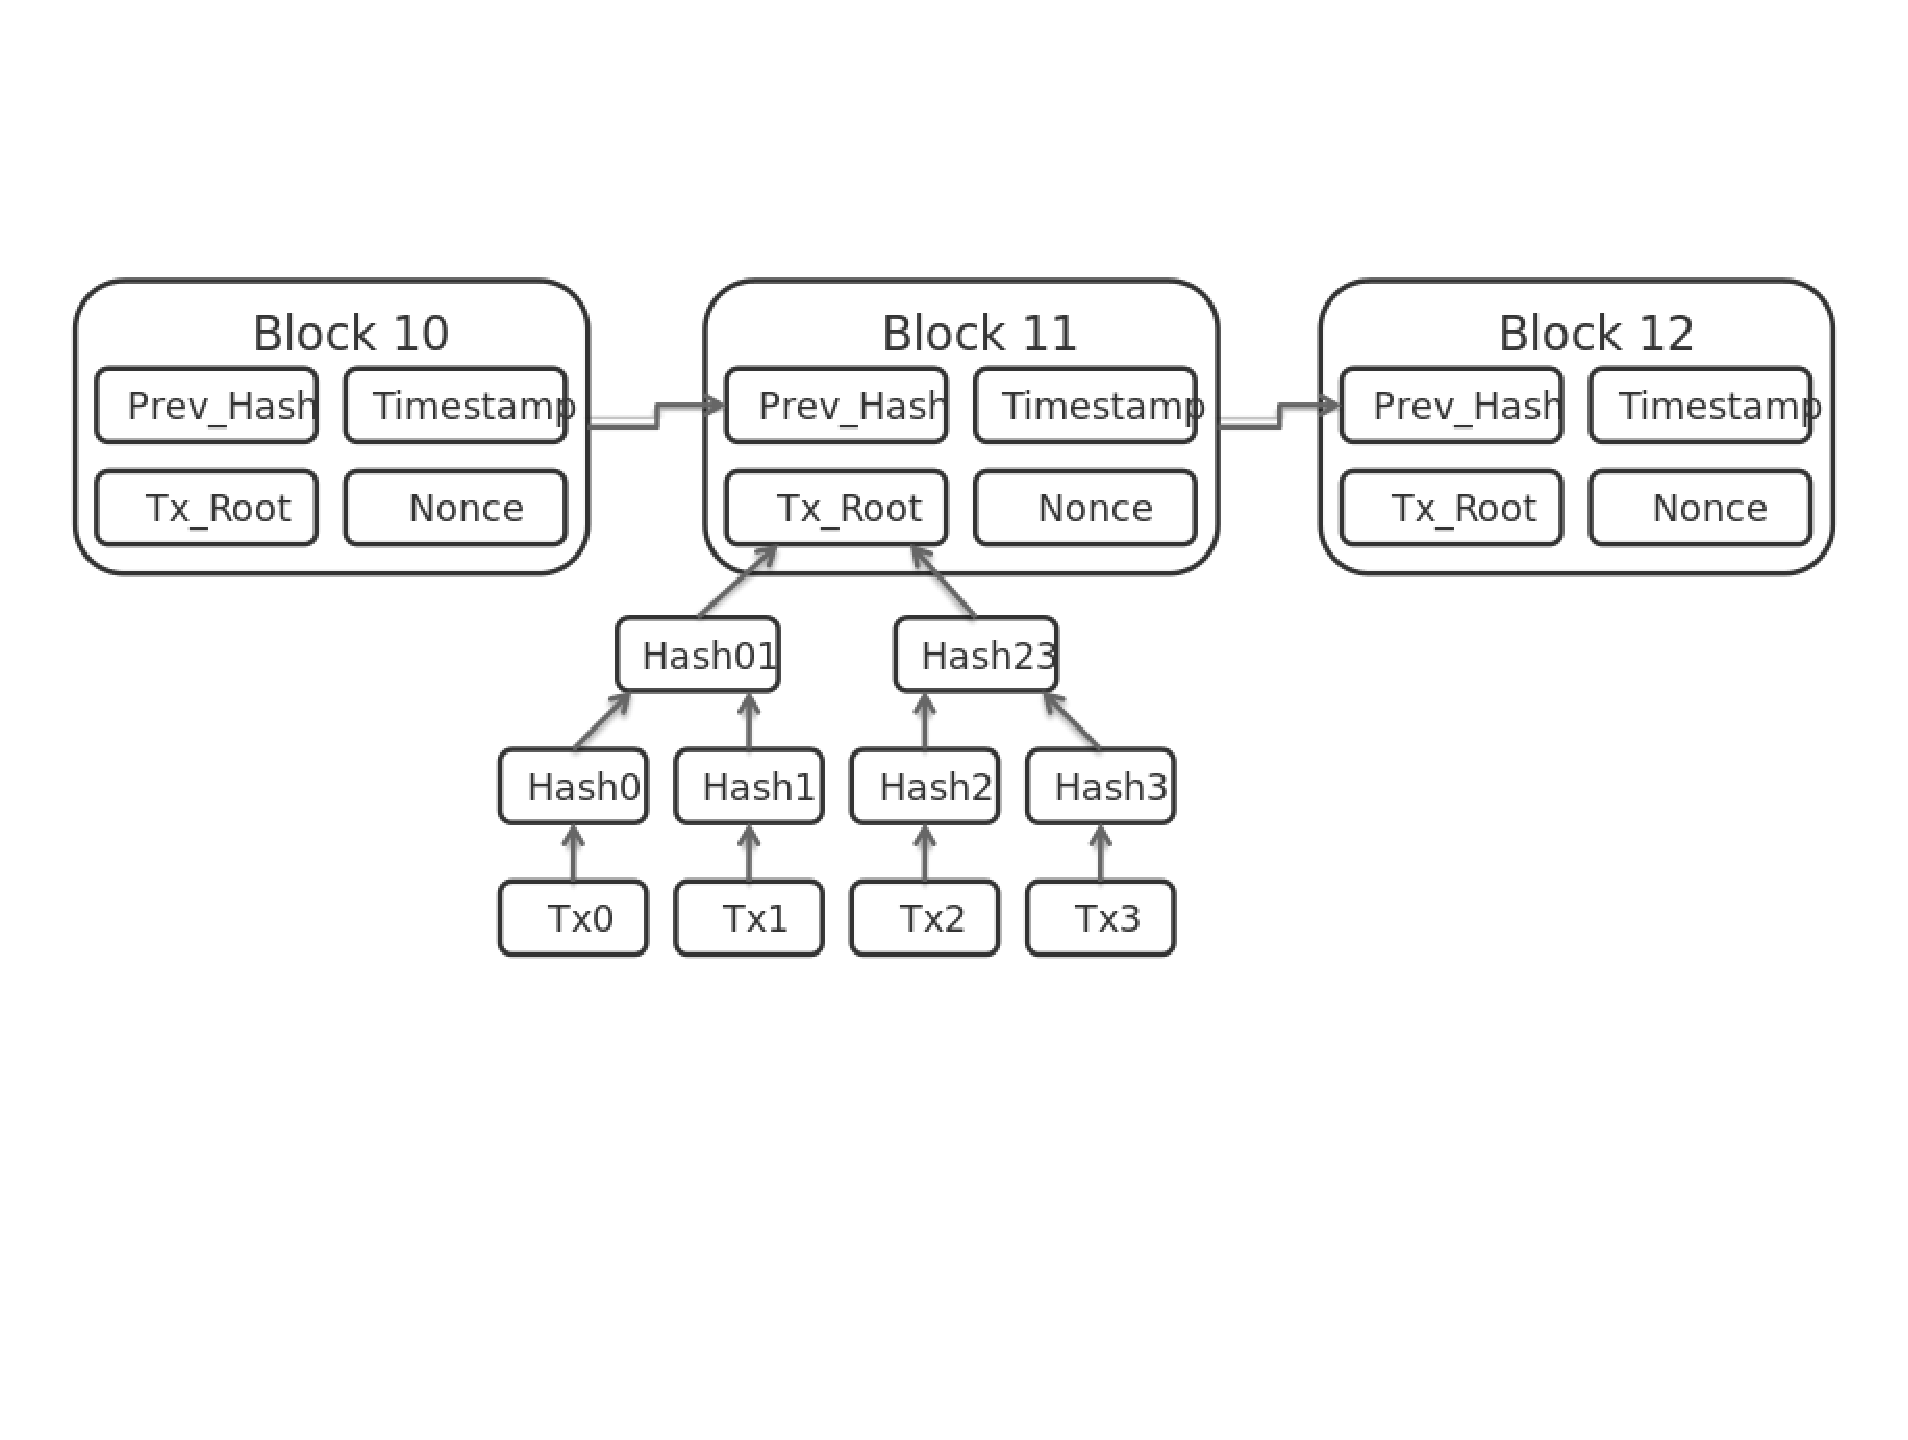
\includegraphics[width=0.7\textwidth]{Images/BlockchainStructure.eps}
	\caption{Blockchain structure taken from~\cite{Bitcoin_Satoshi} }
	\label{BlockchainStructure}
\end{figure}
%Blockchain technology is a variant of distributed database implemented on a P2P
%network. Every participating node in the network has the same copy of history
%of records of the database. Blockchain is essentially a chain of blocks, as the
%name suggests. Each block consists of list of valid transactions (signed
%messages) collected by validators/miners of the network. The linking and
%ordering of transactions are also the responsibility of validators. The
%validators propose a block they have unlocked to the network which can either
%be accepted or rejected. If accepted, the newly created block gets linked to
%the existing blockchain with a hash pointing to the previous block. As such,
%blockchain provides the transaction ordering that every node agreed on at a
%given time. Consensus metric helps to establish and maintain the integrity of a
%blockchain
%system~\footnote{https://github.com/ethereumbook/ethereumbook/blob/develop/consensus.asciidoc}.
%The primary attributes that constitute a blockchain system are distributed,
%decentralized and time-stamped transactions.  There have been P2P protocols
%deployed as a file-sharing or other form of content delivery services before
%Blockchain. What makes Blockchain stand out from them is, for the first time,
%it makes it possible to transfer values online on a P2P network without a
%double-spending problem, i.e., if a peer \textit{'A'} sends a file or a value
%\textit{'v'} to \textit{'B'}, then the file should be owned by \textit{'B'} and
%removed from the account of \textit{A}. \textit{'A'} should not be able to send
%the same file \textit{'v'} to other entities on the network. This was the
%significant contribution of the technology. 
%While, transferring digital contents, sharing information were
%possible before, transferring values was made possible by Blockchain
%technology.
%~\cite{pilkington201611}
%\subsection{Basic Concepts}
%transaction, message, signature, broadcast, verify, network, miners, validate, write blocks 
%~\cite{vwust2017you,oronchenko2017you} provides a detailed discussion on various blockchain
%types and their uses.
\subsection{Consensus Mechanisms}\label{subsec:consensus}
Blockchain, being a distributed database with multiple writers, should have a
way for every node to reach a consensus on a shared global view of the network.
Consensus mechanisms allow doing so. Based on consensus mechanisms, systems can
be distinctly categorized into~\cite{mingxiao2017review}:
\paragraph{\ac{PoW}:}This is the most widely used consensus mechanism in public
permissionless setup. As the name suggests, a validator node (miner node) needs
to provide the proof to the network that it has done a significant amount of
work. This work requires them to invest a substantial amount of computational
resources. The reason for this is that all the validator nodes compete to be
the writer of the next block for which they need to solve a cryptographic
puzzle. The puzzle requires the miners to perform a hash operation on the data
(hash function applied to the concatenation of message and nonce) until the
output hash is less than a specific target value. As the hash function produces
a random output, given an n-bit number, the probability that the
first bit of the generated output hash is 0 is 50 \%, the probability that the
first two bits are 0 is 25 \%, for the first three bits it becomes 12.5\% and
so on. In numeric terms (base 10 number), we can refer to it as the difficulty
of finding a value less than $2^{n-1}$, $2^{n-2}$, $2^{n-3}$ and so on. As such,
lower the target value (also known as difficulty target), lower is the
probability of finding such a value and therefore higher is the difficulty of
the puzzle. The process of repeatedly finding the nonce value until the output
hash satisfies the requirement of being less than a specific target is given by
Figure~\ref{fig:cryptographicPuzzle}. An essential attribute of a hash function
is that a change in even a single bit of input data will completely change the
output hash value.  Therefore, the only way to find a nonce value which when
concatenated with the message will produce an output hash less than the
specified target is via multiple SHA computations until the target is reached.
The first validator node to solve the problem gets to add the proposed block to
the existing blockchain.  In such a system, the selection of the validator node
is random in that anyone among the competing node could be the first to solve
the cryptographic puzzle.  There is no way to know a priori, which node is
going to be the writer of the next block. As such, this consensus mechanism
makes the system DDOS resistant.  However, miners in a \ac{PoW} setup can
decide upon the order of transactions to include in the block although they
cannot modify the transaction data. As such, one may have to wait for few
blocks before having their transactions confirmed and placed into the
blockchain. The transaction order is agreed upon by the network when the
proposed block by validator node is broadcasted and accepted by the network.
The randomness in the cryptographic puzzle makes it rare for two validator
nodes to solve a block at the same time.  However, it is sometimes possible to
reach such a situation leading into several branches of the blockchain. In
which case, the nodes build upon the block that they first received. This
situation gets solved when the next block is solved, and one of the branches
becomes longer over another. In which case, everyone switches to the longest
branch. Given the rarity of such a situation, the blockchain is assumed to be
eventually stabilized. Examples include Bitcoin~\cite{Bitcoin_Satoshi},
Ethereum~\cite{buterin2013ethereum}. 
\begin{figure}
	\begin{center}
	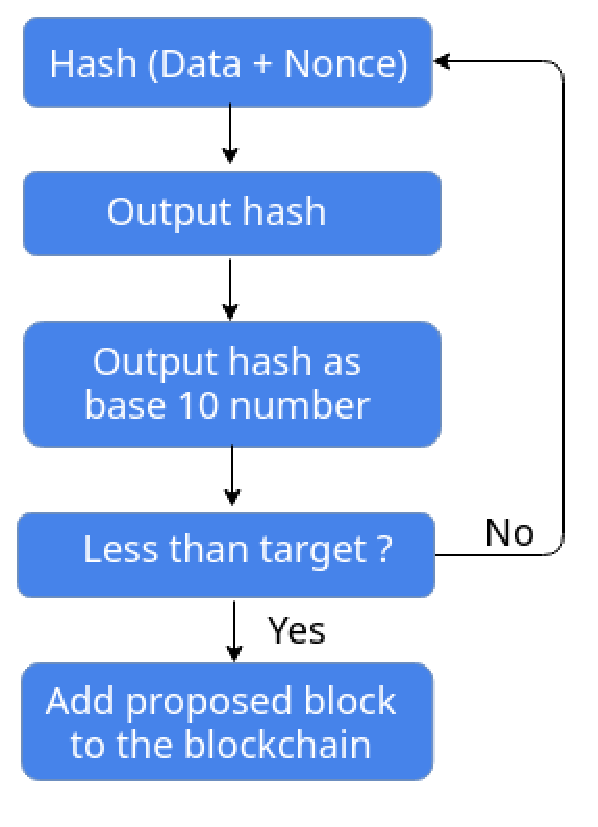
\includegraphics[width=0.4\textwidth]{Images/cryptographicpuzzle.eps}
	\caption{Cryptographic Puzzle}
	\label{fig:cryptographicPuzzle}
	\end{center}
\end{figure}
\paragraph{Economy based systems:}Consensus mechanisms such as \ac{PoS} or
\ac{DPoS} can be seen as an economy based system. Unlike \ac{PoW}, miners do
not compete with each other to be the writer of the next block thus saving lots
of computational resources. The general idea is that participants can put the
respective platform based native token they own at stake to validate a block.
Whoever has the higher value at stake gets to be the writer of the next
block.~\ac{DPoS} differs from ~\ac{PoS} in that, the stakers do not directly
involve in writing a block but rather vote for delegates/witnesses to assign
this responsibility. The elected delegates (node with majority of votes) gets
to write its block to the blockchain. Compared to PoW, it is computationally
efficient as it does not need to invest substantial resources. However, this
also leads to the problem of nothing at stake~\cite{houy2014will}, i.e., a node
could vouch for two forks of the same blockchain. With this setup, a user could
try to double spend the amount they have to two different accounts, and two
different forks would be validating them both. Examples include
Casper~\cite{buterin2017casper}, Ouroboros~\cite{kiayias2017ouroboros}. Casper
solves the problem of nothing at stake by penalizing the node that is detected
to have validated two blocks at the same height.  
%The PoW consensus mechanism, relies on SHA-256 hash (in Bitcoin)
%applied to the block header and nonce to produce a verifiable fingerprint of
%data. This is discussed in more detail in~\ref{sec:blockchain}. Proof-of-work
%was originally used in 1997 by Adam Back as a anti-spam system for the then
%proposed Hashcash~\cite{back2002hashcash}. The general idea being that the
%sender of message would have to compute some number of sha operations before
%sending the message.  The generated fingerprint could be checked by anyone to
%see if the sender has actually done the required number of computations. If a
%legitimate user sending out one email had to spend 'x' seconds to do the sha
%operations, a malicious user intending to send thousands of emails had to spend
%1000x seconds. \\
\paragraph{Leader Based System:}In this case, there is a leader that is
responsible for collecting all the transactions and appending new records to
the blockchain. Having a small group of consortiums, it has low computational
requirements. As a blockchain protocol, it offers an immutable audit of the
records. However, just like any other centralized system, this system is
susceptible to DDOS attacks and third-party (leader) interference. Since the
address of the leader is known to the nodes of the network, it is also known to
the attackers. This form of consensus mechanism is generally used in a private
or permissioned blockchain setup. Examples of blockchain platforms that use
leader based consensus mechanism are Hyperledger
Fabric~\cite{androulaki2018hyperledger}, R3 Corda~\cite{brown2016corda}. In
Hyperledger Fabric, the entire transaction flow (proposal, endorsement,
ordering, validation, and commitment of transactions) is considered to be part
of the consensus algorithm~\cite{hyperledgerfabric,hyperledgerfabric2}, unlike
in other systems where consensus relates to the ordering of transactions. It
makes use of leader election mechanism to elect a leader that is responsible
for ordering transactions. Examples of leader based algorithms are
\ac{PBFT}~\cite{castro1999practical}, RAFT~\cite{ongaro2014search}. 

%\ac{PBFT} comprises of several steps to reach
%consensus which is briefly explained here. The client first makes a request to
%the master server node. The master server node gives a timestamp to the
%request, records the request message and broadcasts a pre-prepare message to
%other server nodes. Other server nodes can either choose to accept or reject
%the request. The server nodes that accept the request will broadcast a prepare
%message to other server nodes and also receive a prepare message from other
%nodes. After having collected 2f+1 messages, if majority of the nodes choose to
%accept the request, then it will enter the commit state. If the server node
%receives 2f + 1 commit messages, then it believes that the nodes reached a
%consensus and executes the instructions in the request message. In the final
%stage, the server nodes only need to send a reply message to the client.
\subsection{Categories}
Along the dimension of validation and access control~\cite{wust2017you},
Blockchain can be categorized as a public permissionless system, public
permissioned, and private permissioned. 
\begin{itemize}
	\item Public Permissionless: Anyone can join the network and become a writer
		of the block as long as they can solve a problem or reach the consensus
		that satisfies the underlying protocol. The records are publicly
		available and thus publicly verifiable. 
	\item Public Permissioned: Anyone can still join the network, but a writer
		of the block is known but not necessarily a trusted entity. The records
		are publicly verifiable. 
	\item Private Permissioned: This is similar to the Public permissioned
		setting, but the records are not made public and therefore does not
		offer public verifiability. This kind of setup is more specific to
		business use-cases where one business does not need to know about other
		business policies or customer information etc. 
\end{itemize}
\subsection{Smart contracts}
A contract in a classical sense is a set of rules with pre-defined obligations
and permissions that participants are assumed to follow. It does not
necessarily need to be legally binding or even associated with the outside
world. The term Smart contact was first coined by Cryptographer Nick Szabo, in
1994~\cite{Szabo1996smart} and defined as a computerized transaction protocol
that can execute the terms of a contract. Szabo points out that the contract
design should fulfill four objectives}: 
%\footnote{https://universe.ida.dk/media/23422289/fritz-henglein.pdf}.
\paragraph{Observability,}ability to observe the contract, performance of
principal (agents who have agreed to the contract) and prove their
performance.
\paragraph{Verifiability,}the ability of principals to prove to the arbitrators
that the contract has been performed or breached.  
\paragraph{Privity,}to ensure that the third party, other than the designated
intermediaries should not have control or knowledge of the content or
performance. It correlates to both privacy and confidentiality of principals of
contract and the contract itself. 
\paragraph{Enforceability,}to make the contract self-enforcing which can be
attributed to by verifiability, built-in incentives mechanism, self-enforcing
protocols. \par
%\begin{itemize}
%	\item \textbf{Observability}, ability to observe the contract, performance of
%		principal (agents who have agreed to the contract) and prove their
%		performance.\\
%	\item \textbf{Verifiability}, the ability of principals to prove to the
%		arbitrators that the contract has been performed or breached. \\ 
%	\item \textbf{Privity}, to ensure that the third party should not have
%		control or knowledge of the content or performance. It correlates to
%		both privacy and confidentiality of principals of contract and the
%		contract itself. \\
%	\item \textbf{Enforceability}, to make the contract self-enforcing which
%		can be attributed to by verifiability, built-in incentives mechanism,
%		and objectives mentioned above. \\
%\end{itemize}
While privity relates to limiting knowledge and control to the third-party, on
the other end, observability and verifiability demand invoking it to an extent.
As such, a trade-off is required wherein an optimal balance between these
objectives should meet. Thus, trusted intermediaries were introduced with
minimal control/observability.  However, privity was not guaranteed in case of
dispute~\cite{szabo1997formalizing}. \par
%Following the invention of Bitcoin and several decentralized blockchains, the
%definition of smart contracts have evolved. 
%To address this, Ethereum introduces the concept of
%gas. To store any state, or execute any operation, gas needs to be supplied.
%Thus, a program that has a bug or a non-terminating intention will eventually
%run out of gas and stop~\cite{whataresmartcontracts}.
\subsection{Ethereum} \label{subsec:ethereum}
Ethereum being the first platform to offer programmable blockchains, introduced
a virtual machine, \ac{EVM}, where the contract code can be executed that
results in a deterministic output provided the same transaction context and
blockchain state~\cite{MasteringEthereum}}. \ac{EVM} often referred to as a
single world computer, runs on every ethereum node and given the same initial
state produces the same final state. Several high level languages can be used
to write smartcontracts for different blockchain platforms. Examples include
solidity~\cite{SolidityDocs}, LLL~\cite{LLL}. The contract code resides in the
blockchain as an immutable form. They are not autonomous self-executing
programs but rather needs to be called by a transaction or invoked by other
contracts. Once the code is registered and deployed on the blockchain, its code
cannot be altered by anyone, including the owner of the contract. However, a
possibility to include a killable function by the owner exists which when
called executes an EVM opcode called SELFDESTRUCT and logically deletes the
contract from the blockchain, i.e., it removes the code and the internal state
from the address of contract. After the deletion of this contract, sending any
transaction to its address will not execute any code. Doing so does not delete
the history of transactions as the blockchain itself is immutable.  As in any
Turing-complete language, it is affected by the halting problem, i.e., there is
no way of knowing if the program will terminate given an input.  In the case of
a non-terminating program, a transaction that is transmitted to the network
might run forever, and the whole network can be rendered useless if
transactions cannot be processed. To avoid this, ethereum introduces the
concept of gas, which is an expendable resource on the network that acts as a
fundamental network cost unit. Gas~\cite{ethereumbiegepaper} is used as a means
to mitigate the possibility of abusing the network with excessive computational
expenditures and is paid for exclusively in ether, which is the unit of
currency in Ethereum. The smallest unit of currency in Ethereum is Wei ($1 Wei
= 10^{-18}$ ether). To store any state, or execute any operation, gas needs to
be supplied. Thus, a program that has a bug or a non-terminating intention will
eventually run out of gas and stop. 
%The Ethereum Protocol~\cite{ethereumbiegepaper} is a deterministic but
%practically unbounded state machine~\footnote{A state machine reads a series of
%inputs and when it reads an input, switches to a different state} with two
%basic functions; the first being a globally accessible singleton state, and the
%second being a virtual machine that applies changes to that state. The globally
%accessible singleton refers to the single global truth of the machine for all
%the transactions created in the system. Ethereum offers a general purpose
%programmable blockchain with a virtual machine that can execute code of
%arbitrary and unbounded complexity. As a distributed state machine, it tracks
%state transitions of a general-purpose data store, where "general purpose data
%store" represents a store that can hold any data expressible as a key-value
%tuple~\cite{MasteringEthereum}. Some of the key components of Ethereum are
%presented below:  


\paragraph{Accounts:}Accounts in Ethereum can be either \ac{EOA} (user account)
which is controlled by the private key of the user or contract account, which
is controlled by code. Every account is associated with a unique identifier
(20-byte hexadecimal number) and has a state. The address of \ac{EOA} is
derived from the last 20 bytes of the keccak-256 hash of the public key. The
contract account, however, is not associated with the public-private key pairs.
There is no private key that owns the contract account. After the contract is
written using a high-level language such as solidity, it can be compiled down
to EVM bytecode, which can then be deployed to Ethereum. The deployment is done
by executing a special transaction namely, CONTRACT CREATION which is sent to a
special address, 0x0. The address of the contract is then derived from the
contract creation transaction as a function of the originating account and
nonce. 


%The nonce is one of four variables that make up the account state each
%of which is discussed below: 
%\begin{itemize}
%	\item{nonce:} The number of transactions sent from this address, or the
%		number of contract creations made by the account associated with this
%		address. 
%	\item{balance:} The amount of Wei owned by this account and is stored as a
%		key/value pair inside the state database~\footnote{A database stored
%		off-chain, i.e., on the computer of some user running an Ethereum
%		client which contains a radix tree mapping byte arrays to byte arrays}.
%	\item{code hash:} The hash of the EVM code of this accounts contract. Code
%		hashes are stored in the state database. Code hashes are permanent, and
%		they are executed when the address belonging to that account receives a
%		message call.  
%	\item{Storage trie root:} A 256-bit (32 bytes) hash of the root node of a
%		Merkle Patricia tree that encodes the storage contents of the account.  
%\end{itemize}
%\paragraph{Transactions:}Transactions are signed messages originated by
%~\ac{EOA}, transmitted by Ethereum network, and recorded on the Ethereum
%blockchain. Transactions can change the state of Ethereum state machine or
%cause a contract to execute in the ~\ac{EVM}. Every transaction has the
%following data field:   
%\begin{itemize}
%	\item gas price: The price of gas (in Wei) to pay the network for a unit of
%		gas. 
%	\item gas limit: The maximum amount of gas to be used while executing a
%		transaction.
%	\item to: The Ethereum address of destination account. In the case of
%		contract creation, this is 0x0. 
%	\item value: The value of Wei to be transferred to the recipient of a
%		message call.
%	\item data: Variable-length binary data payload which can be set by the
%		sender of the transaction. It involves an array of bytes with no limit
%		on length, but more data implies more gas fees. 
%	\item v,r,s: The three components of the ECDSA signature of the originating
%		\ac{EOA}. Using these components, one can derive the public key of
%		\ac{EOA} that signed the transaction message.  
%\end{itemize}
%The global state of Ethereum is a mapping from account addresses to the account
%states which is stored in ~\ac{MPT}.
%


